\documentclass[../main.tex]{subfiles}
\externaldocument{neural_networks}
\externaldocument{kernel_methods}
\externaldocument{../main}



\begin{document}

\section{Clustering Methods} \label{Clustering Methods}
Clustering methods are used to group data when no class labels are present. You thereby want to learn an intrinsic structure of the data.

\subsection{K-Means Clustering}
Goal: Divide data into K clusters so that the variance within the clusters is minimized. The objective function: 

\begin{equation}
    V(D) = \sum_{i=1}^k \sum{x_j \in C_i} (x_j - \mu_i)^2,    
\end{equation}
where $V$ is the variance, $C_i$ is a cluster, $\mu_i$ is a cluster mean, $x_j$ is a datapoint. The algorithm works as follows: 
\begin{enumerate}
    \item Assign the data to k initial clusters
    \item Calculate the mean of each cluster
    \item Assign the data points to the closest cluster mean
    \item If a point changed its cluster, repeat from step 2
\end{enumerate}

\begin{figure}[h]
    \centering
    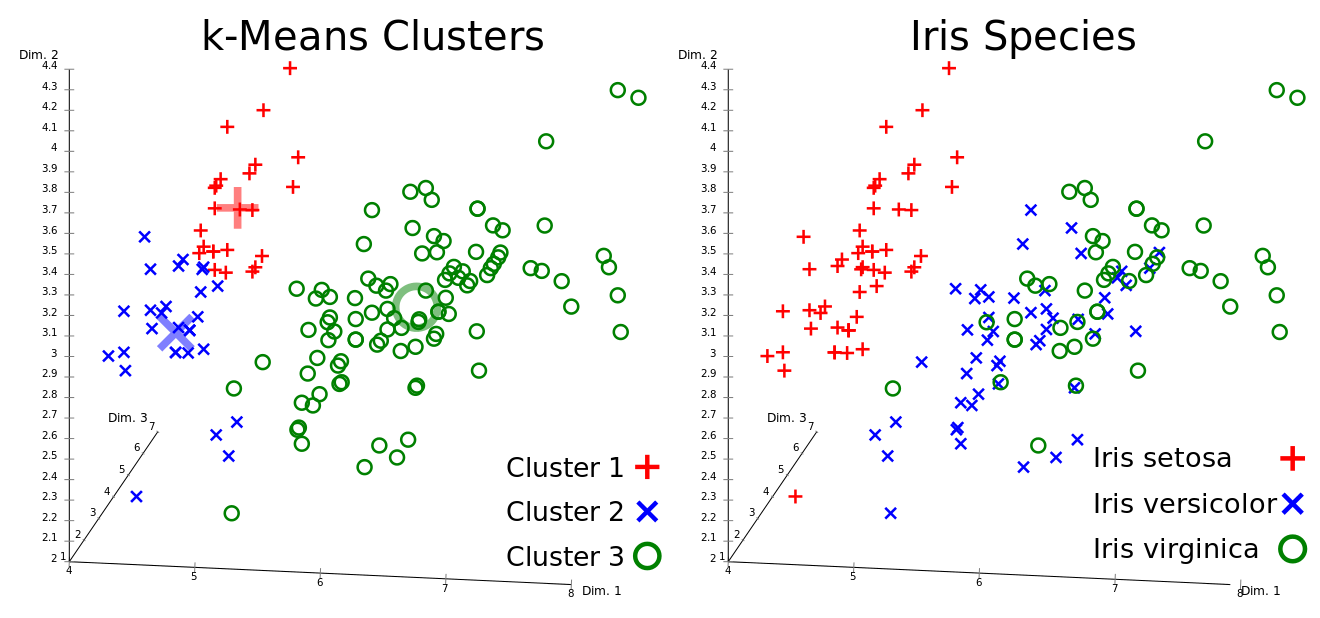
\includegraphics[width=0.6\textwidth]{../figures/kMeans.png}
    \caption{Data from the \textit{Iris flower data set} clustered into 3 clusters using k-Means. On the right the data points have been assigned to their actual species. \textit{Figure from \href{https://commons.wikimedia.org/wiki/File:Autoencoder_schema.png}{user Chire on wikimedia.org}.}}
    \label{CDF}
\end{figure}

\subsection{Graph-Based Clustering}
    You represent data set $D$ as a graph $G=(V,E)$ and divide it up in connected sub-graphs that represent your clusters. Each edge $e_{ij}$ (between nodes $v_i$ and $v_j$) has a weight $w_{ij}$ (which is commonly a similarity or distance measure).

    \paragraph{Basic Graph-Based Clustering} The basic algorithm works like this:
        \begin{enumerate}
            \item Define a weight-threshold $\theta$
            \item For all edges: if $w_{ij}$ > $\theta$: remove $e_{ij}$
            \item If nodes are connected by a path (via \textit{depth first search}): Assign are them to the same cluster
        \end{enumerate}
    \paragraph{DBScan} \textit{Density-Based Spatial Clustering of Applications with Noise} is a more noise robust version of graph-based clustering. 
        
    \paragraph{Cut-Based Clustering} You introduce a \textbf{adjacency/similarity} matrix $W$ (measures similarity between data points) and define the number of clusters $k$. You now try to minimize the weight of edges between the clusters (equal to cutting edges between nodes that are least similar): 

            \begin{align*}
                \begin{split}  
                    \min \frac{1}{2} \sum_{a=1}^k \sum_{b=1}^k \kappa(C_a, C_b) \\
                    \text{where } \kappa(C_a, C_b) = \sum_{v_i \in C_a , v_j \in C_b , a \neq b} W_{ij} \\ 
                    \text{ and } \kappa(C_a, C_a) = 0
                \end{split}
            \end{align*}
            $\rightarrow$ You only add up the similarities/edge-weights between your clusters (but not within your clusters). \\
            \btw For constructing the similarity matrix, different kernels can be used (commonly the linear kernel or the Gaussian kernel).

\subsection{Spectral Clustering} \label{Spectral Clustering}
The goal is again, to cluster the points, such that the similarity of points of different clusters is minimal. Spectral clustering employs three steps: Preprocessing, decomposition and grouping. 
\paragraph{Preprocessing} We create a Laplacian matrix $L$ (laplacian operator in matrix form, measuring how strongly a vertex differs from nearby vertices (because the edges are similarity measures)): %todo is it really differs or rather similar 
    $$L = D - W$$  
    \[ D_{ij} = \begin{cases}
        \sum_{j=1}^N W_{ij} \\ 
        0 \text{ if } i \neq j
    \end{cases} \]
    where $D$ is the degree matrix (the degree of each node is on the diagonal). 
\paragraph{Decomposition} The class assignment is encoded in vectors $c_k$. We normalize them and get e.g.: 
    \[ u_a = \frac{c_a(i)}{||c_a||}  = \begin{cases}
            \frac{1}{||c_a||} \text{ if } v_i \in C_a \\
            \frac{0}{||c_a||} \text{ if } v_i \notin C_a \\
        \end{cases}\]
    As in cut-based clustering we search for a minimum k-cut, but also add a constraint that $u_a^T u_a = 1$ 
    $$
    \min \frac{1}{2} \sum_{a=1}^k u_a^T L u_a + \lambda_a \sum_{a=1}^k 1-||u_a||^2
    $$
    We find the optimal $u_a$ by eigenvalue decomposition:
    $$
    L u_a = \lambda u_a
    $$
    The final data is now represented as a matrix of k eigenvectors (of the least dominant eigenvalues) as column-vectors. 
    
\paragraph{Grouping} You get the final cluster assignments by normalizing the now k-dimensional data and applying k-means clustering to it. 

\subsubsection{Sparse Subspace Clustering (SSP)} \label{SSP}
The underlying assumption of SSP is that the different clusters reside in different subspaces of the data. Clusters are therefore perpendicular to each other and points in a cluster can only be reconstructed by combinations of points in the same cluster ($\rightarrow$ self-expressiveness, the reconstruction vectors ought to be sparse). For each point you try to find other points that can be used to recreate that point - these then form the same cluster. Doing that for all points gives you a data matrix $X$ and a matrix of reconstruction vectors $V$:

        $$
        X = X*V\text{ s.t. diag}(V)=0.
        $$

        You now try to minimize the V-matrix according to the L1-norm (giving you a sparse matrix). This matrix can then be (multiplied with its transpose and) used for e.g. spectral clustering.

\subsection{Soft-assignment Clustering}

    \subsubsection{Expectation Maximization (EM) Clustering}
    \textit{[Coming soon]}

    \subsubsection{Gaussian Mixture Models}
    \textit{[Coming soon]}



\subsection{Artificial Neural Networks for Clustering}
    See chapter \textit{Neural Networks} (\ref{Neural Networks})
\end{document}
